\chapter{Intersection graphs of paths on grid and trees}\label{Notions}

\vspace{2.5cm}
\begin{flushright}
\begin{minipage}[t][0cm][b]{0.47\textwidth}
\emph{%Se você conhece o inimigo e conhece a si mesmo, não precisa temer o resultado de cem batalhas. 
If you know the enemy and know yourself, you need not fear the result of a hundred battles. If you know yourself but not the enemy, for every victory gained you will also suffer a defeat. If you know neither the enemy nor yourself, you will succumb in every battle.
}
\end{minipage}

\rule[0cm]{7cm}{0.03cm}%{largura}{espessura}

Sun Tzu, The Art of War
\end{flushright}

\begin{quotation}
In this chapter, we will present some concepts that will facilitate the understanding of the studied problems. In particular, we describe the notations and we will illustrate with examples only those concepts and definitions that are outside the basic scope of graph theory. As a basic bibliography on graphs, algorithms, and NP-completeness we suggest reading~\cite{bondy1976graph} and~\cite{jayme2018} .
\end{quotation}
%\section{Preliminaries}

In this thesis, we will consider finite graphs, connected and simple, i.e. graphs without loops (edge connecting a vertex in itself) or more than one edge connecting two vertices. Thus, when we talk about graphs we will consider a simple, finite and connected graph unless something different is explicitly said.

Next, we describe the terminology and notation used in this work.

A \emph{graph} $ G $ is a structure composed of two finite sets: $ V(G) $ is a non-empty set whose elements are called \emph{vertices}, and $ E(G) $ is a set of unordered pairs of distinct elements taken from $ V(G) $, which are called \emph{edges}. An edge $ e=(u, v) \in E (G) $ is formed by the pair of vertices $ u, v \in V(G) $, in this case $ u $ and $ v $ are said to be vertices \emph{adjacent}. We also say that $ e $ is \emph{incident edge} to $ u $ and $ v $. We denote the \emph{cardinality} of $ |V(G)| = n $ and $ |E(G)| = m $.

Given a vertex $v\in V(G)$,  $N(v)$ and $N[v]$ represent the \emph{open} and the  \emph{close neighborhood} of $v$ in $G$, respectively. 
For a subset $S \subseteq V(G)$,  $G[S]$ is the subgraph of $G$ induced by $S$.
 If $\mathcal{F}$ is any family of graphs, we say that  $G$ is  \emph{$\mathcal{F}$-free} if $G$ has no induced subgraph isomorphic to a member of $\mathcal{F}$.


Let $u, v$  be vertices of $G$, if $N(u) = N(v)$ then $u$ and $v$ are said \emph{false twins}, on the other hand, if $N[u] = N[v]$, then $u$ and $v$ are said \emph{true twins}. The \emph{degree of a  vertex} $v$ is denoted  by $d(v)$ and corresponds to the number of vertices adjacent to $v$, i.e., the cardinality of $|N(v)|$. The \emph{maximum degree} of a graph $G$ is denoted by $\Delta(G) = \max\{d(v) \mid v \in V(G)\}$. Similarly, the  \emph{minimum degree} is denoted by  $\delta(G) = \min \{d(v) \mid v \in V(G)\}$.

Given a graph $G$, and a vertex $v \in V(G)$, the graph $G\backslash \{v\}$ is obtained from $G$ by removing the vertex $v$ from its vertex set, and also removing all edges of $E(G)$ incidents at $v$. Similarly, given an edge $e \in E(G)$, the graph $G\backslash \{e\}$ is obtained from $G$ removing the edge $e$ from $E(G)$.

We say that $G'=(V',E')$ is a \emph{subgraph} of a graph $G=(V,E)$ when $V'\subseteq V$ and $E'\subseteq E$. When the subgraph $G'$ contains all edges of $E$ whose ends are contained in $V'$, then  $G'$ is the \emph{induced subgraph} of $G$ by $V'$.  

A graph  $G$ is a \emph{cycle}, denoted by $C_n$, if it is a sequence of vertices   $v_1, \dots, v_n, v_1$, where $v_i \neq v_j$ for $i\neq j$ and $(v_i, v_{i+1})\in E(G)$,  such that $n\geq 3$. For a cycle $C_k$, we say that it is an
\emph{even cycle} if $k$ is even and an \emph{odd cycle}, otherwise. A \emph{chord} is an edge that is between two non-consecutive vertices in a sequence of vertices of a cycle. An \emph{induced cycle}  or \emph{chordless cycle} is a cycle that has no chord. A graph that has no cycles is called \emph{acyclic}. A  graph $ G $ is \emph{connected} if there is a path between any pair of  vertices of $ G $. A graph is a \emph{tree} when it is acyclic and connected. A connected subgraph of a tree is called \emph{subtree}.

A set $\mathcal{S}$ is \emph{maximal} in relation to a particular property $P$ if $\mathcal{S}$ satisfies $P$, and each set $S'$ containing properly $\mathcal{S}$ does not satisfy $P$. In a similar way, a set $\mathcal{S}$ is \emph{minimal} in relation to a particular property $P$ if $\mathcal{S}$ satisfies $P$, and each subset  $S'$ that is properly contained in $\mathcal{S}$ does not satisfy $P$.

A graph $G$ is a \emph{intersection graph} of a family of subsets of a set $\mathcal{S}$, when it is possible to associate each vertex $v \in V(G)$ to a subset $S_v \subseteq \mathcal{S}$, such that $S_u \cap S_v \neq \emptyset$ if and only if $(u,v)\in E(G)$.  In this thesis, in particular, we will study four families of intersection graphs: the VPG, EPG, VPT and EPT graphs.


The term \emph{grid} is used to denote the Euclidean space of entire orthogonal coordinates. Each pair of entire \emph{coordinates} corresponds to a point or \emph{vertex of the grid} (which by the context is not to be confused with the vertex of the graph). The term \emph{grid edge} (which is also not to be confused with the edge of the graph), will be used to denote a pair of vertices that are at distance one in the grid. Two edges $ e_1 $ and $ e_2 $ are \emph{consecutive edges} when they share exactly one point on the grid. A grid is the \emph{host} on which we accommodate the VPG and EPG representations. When we refer to the VPT and EPT graphs, we implicitly know that the host of their representations is a tree.



 A \emph{path in the grid} is distinguished by two contexts, in the first we study families of subsets $\cal{F}$ of edge of the grid. In this context a path in the grid is defined as a finite sequence of consecutive edges  $e_1 = (v_1, v_{2}), e_2 = (v_2, v_{3}), \dots, e_i = (v_i, v_{i+1}), \dots, e_m = (v_{m}, v_{m+1})$,  where   $v_i \neq v_j$ for $i \neq j$.  We call a collection of such paths an {\it EPG representation}, i.e., a collection of paths that represent a graph via its intersection graph (considering edge intersections). {\it EPG graphs} are the class of graphs that admit an EPG representation.
  In the second context, for vertex paths, we study families of subsets $\cal{F}$ of vertex of the grid, and a path consists of a sequence of consecutive vertices of the grid  $v_1, v_2, \dots , v_k$ such that $(v_i, v_{i+1})$ is an edge of the grid, for all $i \in {1, \dots,  k - 1}$, where   $v_i \neq v_j$ for $i \neq j$, and a collection of these paths forms a {\it VPG representation} and corresponds to a {\it VPG graph}. 

 
 The first and last edges of a path are called \emph{extremities edges}.
The \emph{direction of an edge} is \emph{vertical} when the first coordinate of its vertices is equal, and is \emph{horizontal} when the second coordinate is equal. A \emph {bend} in a path is a pair of consecutive edges $ e_1, e_2 $ of the path, such that the directions of $ e_1 $ and $ e_2 $ are different. When two edges $ e_1 $ and $ e_2 $ form a bend, they are called \emph{bend edges}. A \emph{segment} is a path without bend.
 
 In context of EPG graphs, we say that two paths are
 \emph{edge-intersecting}, or simply  \emph{intersecting}, if these share at least one edge (of the grid).
 
 
 EPG graphs are a class of  intersection graphs of paths on a grid~\cite{golumbic2009}. Shortly after came the VPG graphs, this class was introduced in 2011 \cite{asinowski2011string} and \cite{asinowski2012}. 
 These classes consist of graphs whose vertices can be represented by paths of a grid $ Q$, such that two vertices of $ G $ are adjacent if and only if the corresponding paths intersect (in edges, if EPG graphs or in vertex, if VPG graphs). If every path in a representation can be represented with a maximum of $ k $ bends, we say that this graph $ G $ has a  \emph{$ B_k$-EPG} (resp. \emph{$ B_k$-VPG}) representation. When $ k = 1 $ we say that this is a \emph{single bend} representation.

 Let $P$ be a family of paths on a host tree $T$ . Two types of intersection graphs from the pair $<P,T>$ are defined, namely VPT and EPT graphs.
The \textit{edge intersection graph} of $P$, EPT(P), has vertices which correspond to the members of $P$, and two vertices are adjacent in EPT(P) if and only if the corresponding paths in $P$ share at least one edge in T. Similarly, the \textit{vertex intersection graph} of $P$, VPT(P), has vertices which correspond to the members of $P$, and two vertices are adjacent in VPT(P) if and only if the corresponding paths in $P$ share at least one vertex in $T$.
%
VPT and EPT graphs are incomparable families of graphs. However, when the maximum degree of the host tree is restricted to three the family of VPT graphs coincides with the family of EPT graphs \cite{golumbic1985edge}. Also, it is known that any Chordal EPT graph is VPT (see~\cite{syslo1985triangulated}). Recall that it was shown that Chordal graphs are the vertex intersection graphs of subtrees of a tree \cite{gavril1974intersection}.
% \cite{alcon2010necessary

We say that a family  $\mathcal{F}$ of sets is \emph{$k$-intersecting} if for each $F_1, F_2, \dots, F_k$ subsets of $\mathcal{F}$, we have that $F_1\cap F_2 \cap \dots \cap F_k \neq \emptyset$. We also say that a family $\mathcal{F}$  of sets is \emph{$k$-Helly}, when every subfamily $k$-intersecting $F'$ of  $\mathcal{F}$ has at least one common element.
 In particular, we say that a family of sets is \emph{pairwise intersecting}, i.e. two by two intersecting if any two sets in the family intersect. A collection $ C $ of non-empty sets satisfies the Helly property, i.e. it is $ 2$-Helly, when every subcollection pairwise intersecting $ S $  of $ C $ has at least one element that is in every subset of $ S$.

For simplicity of notation, in this thesis when we refer to a family of sets as a Helly family it is understood that this family is $ 2$-Helly.

In Boolean algebra, a \emph{clause} is a disjunction or conjunction of literals. We say that a \emph{formula} $ F $ is in the \emph{Conjunctive Normal Form} (CNF) if $ F $ is a conjunction of clauses, where a clause is a disjunction of literals.

\section{Related Works}

In this section, we will present the main known results on the related study topics in this work, namely Helly property, EPG, VPG, EPT, and VPT graphs.

\subsection{On the Helly property}


The Helly property is named in honor of the Austrian mathematician Eduard Helly, who in 1923 proposed a famous theorem about the relationship of intersecting sets. Such a theorem motivates the so-called \textit{Helly property} which can be  stated as follows: given a collection of  sets $ C$, not empty, we say that this collection satisfies the Helly property when every subcollection of $C$ that is pairwise intersecting has at least one element in common.


We can note that the Helly property is a topic that has instigated scientific research since it appeared, moreover, we can also mention recent works in the area of Graph Theory, see~\cite{berge1973, bergeDuchet1975, DOURADO2008, golumbic2013, dourado2006computational, teles2016, jose2018}.
The study of the Helly property proves to be useful in the most diverse areas of science, of which one can enumerate applications in semantics, code theory, computational biology, database, image processing, graph theory, optimization, in problems of location and linear programming, \cite{teles2016}. In particular, in the area of Graph Theory, the Helly property has motivated the study of several graph classes, for example, we can cite the  Clique-Helly graphs~\cite{DOURADO2008}, Helly Circular-arc~\cite{safe2016essential}, Helly EPT~\cite{alcon2017helly}, Disk-Helly~\cite{lin2007faster} and Helly Hypergraphs~\cite{mulder1979median}.


In addition to the applications mentioned above, the Helly property can be studied on  $ B_k$-EPG representations, where each path is considered as a set of edges. A  graph $ G $ has a Helly-$B_k$-EPG representation if there is a $ B_k$-EPG representation of $ G $ where each path has at most $ k $ bends and the representation satisfies the Helly property.
We will use the  notation $ P_{v_i} $ to indicate the path corresponding to the  vertex $ v_i$.
Figure~\ref{fig:envelopeRepresentacoes}(a) depicts two representations $ B_1$-EPG of a graph with 5 vertices. Figure~\ref{fig:envelopeRepresentacoes}(b) depicts pairwise intersecting paths ($ P_{v_1}, P_{v_2}, P_{v_5} $), containing a common edge, so this is a  Helly-$B_1$-EPG representation. In Figure~\ref{fig:envelopeRepresentacoes}(c), although the 3 paths are pairwise intersecting, there is no edge common to the 3 paths simultaneously, and thus they do not satisfy the Helly property.


\begin{figure}[h]
  \centering
  \begin{tabular}{ p{3.2cm} p{4.5cm} p{4.5cm} }
    \centering 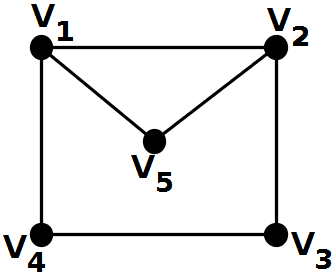
\includegraphics[width=3cm]{./img/envelope} & 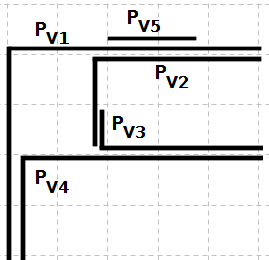
\includegraphics[width=4cm]{./img/envelopeHellyGradeTransparente} & 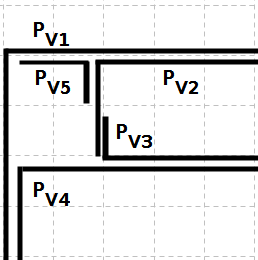
\includegraphics[width=4cm]{./img/envelopeNaoHellyGrade}
    \\
    \footnotesize \centering (a) A  graph with 5 vertices. & \footnotesize(b) A $B_1$-EPG representation that satisfies the Helly property. & \footnotesize (c) A $B_1$-EPG representation that does  not satisfy the Helly property.  \\

  \end{tabular}
\caption{A  graph with 5 vertices in (a) and some single bend representations: Helly in (b) and not Helly in (c).} \label{fig:envelopeRepresentacoes}
\end{figure}

%%%%%%%%%%%%%%%%%%%%%%%%%%%%%%%%%%%%%%%%%%%%%%%%%%%%%%%%%%%%%

In this thesis, we are interested in EPG representations of graphs that satisfy the Helly property. In particular, for the $ B_1$-EPG graphs, this directly implies that each clique has a special format, and the paths that compose it always share an edge of the representation in the grid, i.e. an edge-clique. Using this premise we were able to present Helly subfamilies for $ B_1$-EPG graphs and we also presented a hardness proof  in recognizing this class of graphs.
 We will also study within the scope of this research the parameters Helly number and strong Helly number in paths on a grid.

\subsection{On EPG graphs}

A problem related to the study of EPG graphs is the problem of edge-intersection graphs of paths in a tree, well known in the literature as EPT (Edge-intersection Graphs of Paths in a Tree), see for instance~\cite{gavril1974intersection, golumbic2004recognition}. For EPT graphs, in particular, the value of the parameters Helly number, which is 2, and the strong Helly  number, which is 3, are known results, also in~\cite{golumbic2004recognition}. The parameters Helly number and strong Helly number had been studied in EPT graphs when the set of paths satisfies the Helly property, see
~\cite{petito2002grafos} and \cite{petito2009grafos}.

Regarding the complexity of the $B_k$-EPG graph recognition, only the hardness recognition of a few of these graph subclasses was determined.  $ B_0$-EPG can be recognized in polynomial time, since these correspond to the interval graphs, see~\cite{booth1976}. In contrast, the $ B_1$-EPG and $ B_2$-EPG graphs recognition are $ NP$-complete problems, see~\cite{heldt2014, martin2017}, and the $ B_1$-EPG graph recognition problem remains $ NP$-complete even  for $ L$-shaped paths on a grid, see~\cite{cameron2016edge}. Moreover, in this doctoral thesis you will also find an $ NP$-completeness proof  for the  Helly-$B_1$-EPG graphs recognition in Chapter~\ref{cap:capiii}, and the same chapter we further studied the subsets of $L$-shapes and its relationship with $B_1$-EPG and Helly-$B_1$-EPG graphs.

In this work, we are going to study graphs that have a Helly-EPG representation and related subjects.  The Helly property related to EPG graph representations was studied by~\cite{golumbic2009} and~\cite{golumbic2013}. In particular, they determined the parameter strong Helly number of graphs $ B_1$-EPG. We determine two parameters to every class of EPG graphs, the Helly number and strong Helly number, these results are presents in Chapter~\ref{cap:iv}.

Research about graphs of edge-intersection of  paths on a grid is a relatively new topic in the area of Graph Theory. The first formal definitions of problems and applications were presented by Golumbic in 2009~\cite{golumbic2009}. Since then, several branches of researches have been conducted by the scientific community. These questions often discuss the path representations, restrictions on the bend number in a representation, among others. 
A survey that summarizes the state-of-the-art for the topic of EPG graphs can be found at~\cite{chung201950}. 

Next, we present  some results regarding the  \emph{bend number} for some classes of graphs, among others.

In their study, \citeauthor{alcon2016}~\cite{alcon2016}, the authors show that 3 bends are enough to represent all graphs in the class of circular-arc graphs, i.e. they are in $ B_3$-EPG. Additionally, they also show that there are circular-arc graphs that cannot be represented with 2 bends. Using the fact that we can to represent any circular-arc graph using only a rectangle of a grid of any size, the work defines the class of EPR graphs and classifies the normal circular-arc graphs  as being $ B_2$-EPR, they also show that there are normal circular-arc graphs that are not $ B_1$-EPR. Finally, the work gives a characterization of $ B_1$-EPR graphs by a minimal family of forbidden induced subgraphs and shows that this subfamily corresponds to a subclass of normal Helly Circular-arc graphs.


In the paper of ~\citeauthor{biedl2010}~\cite{biedl2010}, the authors show that 5 bends are enough to represent all planar graphs and that 3 bends are enough to represent all outerplanar graphs. These results are further improved by~\cite{daniel2014b}. In addition to these results, the work shows that every Bipartite Planar graph has a $B_2$-EPG representation and that every Line graph has a $B_2$-EPG representation. In this thesis, we demonstrate that every Line of Bipartite graph is in Helly-$B_1$ EPG, these results are in Chapter~\ref{cap:v}.

\citeauthor{daniel2014b} in~\cite{daniel2014b} showed that 4 bends are enough to represent all planar graphs and present a linear algorithm to find this representation with 4 bends. However, the authors still comment that for some planar graphs, 3 bends are often enough to construct the representation. In fact, it is not that simple the majority of planar graphs could be constructed with 4 bends, in fact, there are no known planar graphs that cannot be drawn using 3 bends. This leaves the question: if 4 bends are always enough to represent any planar graph, then are 4 bends really needed to represent any planar graph? That question is still open. The authors still conjecture that there is a graph where for any of its EPG representations there is always at least one path that needs to use the 4 bends.


The Table~\ref{tab:limitesBenNumber} presents the main known bounds for the \emph{bend number}, denoted by $b(G)$, of some graph classes.


\begin{table}[h]
\caption{Some graph classes and  known bounds to their \textit{bend number}.}
\label{tab:limitesBenNumber}
\begin{center}
\begin{tabular}{|c|c|c|}
\hline 
Graph Class & b(G) & Reference \\ 
\hline \hline  
Interval graphs & 0 & \cite{golumbic2009} \\ 
\hline 
Forests, Cycles & 1 & \cite{golumbic2013} \\ 
\hline 
Outerplanar &  2 & \cite{daniel2014b} \\ 
% \hline 
% Planar & 5 e dim $(n-1)\times(2n-3)$ & \cite{biedl2010} 2010\\ 
\hline 
Planar & $\in [3, 4]$ & \cite{daniel2014b}\\ 
\hline  
  Bipartite Planar & 2 & \cite{biedl2010} \\ 
\hline 
Line Graph & 2 & \cite{biedl2010} \\ 
\hline 
dgn(G)~\footnotemark %\footnote{Degeneracy}
$\leq k$ & $2k-1$ & \cite{daniel2014b} \\ 
\hline 
tw(G)~\footnotemark%\footnote{Treewidth} 
$\leq k$ & $2k-2$ & \cite{daniel2014b} \\ 
\hline 
Degree $\leq \Delta$ & $ \in [	\lceil \frac{\Delta}{2}\rceil, \Delta ] $ & \cite{daniel2014b} \\ 
\hline 
Circular-arc & 3 & \cite{alcon2016} \\ 
\hline 
Normal Circular-arc & 2 & \cite{alcon2016} \\ 
\hline 
Halin graphs & 2 & \cite{mathew2016}  \\ 
\hline 
\end{tabular} 
\end{center}
\end{table}



\footnotetext[1]{Degeneracy}
\footnotetext[2]{Treewidth}
% \footnotetext{Degeneracy}
% \footnotetext{Treewidth}

In addition to the results cited for bounds on the bend number of some classes of graphs, there are many works that characterize other types of graphs not mentioned in this table, such that the work of~\citeauthor{ries2009} in~\citep{ries2009} that characterizes the Chordal graphs  claw-free, bull-free and diamond-fee that have a $ B_{1}$-EPG representation. In that same article, there is also a characterization of some Split graphs, with a restriction on the size of the independent set or  clique, by forbidden subgraphs. The work still has an interesting result that shows that the neighborhood of every vertex of a graph $ B_1$-EPG induces a graph that is Weakly Chordal. Implicitly this paper delimits a set of Helly-$B_1$-EPG graphs, the bull-free graphs. Based on this fact in this thesis, we extend the results to delimit another Helly-$B_1$-EPG subfamily, the diamond-free subfamily. This result can be found in Chapter~\ref{cap:v}.

Although it is possible to find several lines of researches on EPG graphs investigating the bend number, the interests of studies in this class of graphs extend to other classic problems, which we can mention to follow.


In~\citet{cohen2014} a linear time recognition algorithm is presented for $ B_{1}$-EPG Cographs by a family of forbidden induced subgraphs. The algorithm that the paper presents uses the Cotree of the Cograph in the recognition process.

Approximation Algorithms for colorize $ B_1$-EPG graphs  were studied in~\cite{epstein2013approximation}. The work cited shows that the coloring problem and the maximum independent set problem are both $ NP$-complete for graphs $ B_1$-EPG even when the EPG representation is given. The authors present a 4-approximate algorithm that solves both problems, assuming that the EPG representation is given. The work still shows that the maximum clique can be found efficiently in graphs $ B_1$-EPG even when the representation is not given.

Clique coloring problems in $B_1$-EPG graphs were studied by~\cite{bonomo2017clique}. The authors consider the clique coloring problem and show that $B_1$-EPG graphs are 4-clique-colorables and present a linear time algorithm to solve the problem. Moreover, given a $B_1$-EPG representation of a graph, the paper provides a linear time algorithm that constructs a 4-clique coloring of it.
 
We can also mention as an often research with respect to EPG graphs the study of $NP$-hardness~\cite{daniel2014b, martin2017}, area of the grid necessary to represent a graph whose maximum degree is $\Delta(G)$~\cite{Asinowski2009}, and many others. The hardness of recognizing few classes of EPG graphs is known, and even for small $ k $ values only. Research with EPG graphs whose representations satisfy the Helly property is sparse. Thus, these topics and other similar topics prove to be interesting branches of research from a scientific point of view.

Finally, we mention that the $B_k$-EPG hierarchy is proper, i.e.,

$B_0$-EPG $\subset$ $B_1$-EPG $\subset$ $B_2$-EPG $\subset \dots$ $B_{k-1}$-EPG $\subset$ $B_k$-EPG $\subset$ $B_{k+1}$-EPG 

this result is demonstrated by~\citet{biedl2010} for even $k$ and  \citet{heldt2014} complete the result for all $k$.
A correlated result is presented by~\citet{Asinowski2009} that proved that for any $k$, only a small fraction of all labeled graphs on $n$ vertices are $B_k$-EPG.

\subsection{On VPG graphs}

VPG representations arise naturally when studying circuit layout problems
and layout optimization where layouts are modeled as paths (wires) on
grids. One approach to minimize the cost or difficulty of production involves minimizing the number of times that each path bend, see~\cite{bandy1990, molitor1991, sinden1966topology}.
Other times layout may consist of
several layers where the paths on each layer are not allowed to intersect. This is naturally modeled as the coloring problem on the corresponding intersection graph, see~\cite{Alcn2017VertexIG}.


A graph is a VPG if it is the vertex intersection graph of paths in a grid. A graph is called
$B_k$-VPG if it has a $B_k$-VPG representation, i.e. if there is a representation where each path in this representation has at most $k$ bends. VPG graphs were introduced in 2011 by~\citet{asinowski2011string} and~\citet{asinowski2012}. They prove that VPG and String are
the same graph class. However, it is known that  recognizing String graphs is an $NP$-complete problem, by the results of~\cite{schaefer2003recognizing, kratochvil1991string}.

\citet{asinowski2012} study $B_0$-VPG graphs and observe
that horizontal and vertical segments have strong Helly number 2 and that the clique problem has polynomial-time complexity, given the path representation. Among other results, they present proof that the recognition and coloring problems for $B_0$-VPG graphs are $NP$-complete. Moreover, they  give a 2-approximation algorithm for coloring $B_0$-VPG graphs. Furthermore, they prove that triangle-free $B_0$-VPG graphs are 4-colorable, and this is best  possible. In addition, they present a hierarchy of VPG graphs relating them to other known families of graphs, see Figure~\ref{fig:hierarquiaVPG}. The grid intersection graphs are shown to be equivalent to the bipartite $B_0$-VPG graphs and the circle graphs are strictly contained in $B_1$-VPG. They still prove the strict containment of $B_0$-VPG into $B_1$-VPG, and conjecture that, in general, this strict containment continues for all values of $k$. Finally, they present
a graph that is not in $B_1$-VPG. 

\begin{figure}[htb]	
\center%6.3
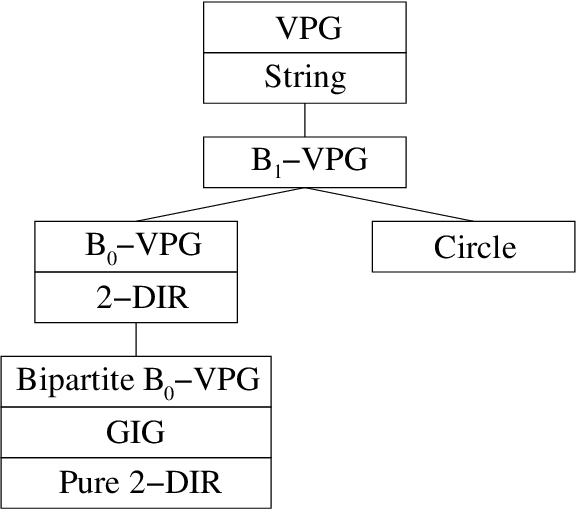
\includegraphics[width=6cm]{./img/hierarquiaVPG.png}
\caption{Relations between $B_k$-VPG graphs and well known graph classes \cite{asinowski2012}. }
\label{fig:hierarquiaVPG}
\end{figure}


It is known that all planar graphs are $B_2$-VPG, see~\cite{chaplick2012planar}. This paper also shows that the 4-connected planar graphs constitute a subclass
of the intersection graphs of $Z$-shapes (i.e., a special case of $B_2$-VPG). Additionally, they demonstrate that a $B_2$-VPG representation of a planar
graph can be constructed in polynomial time. They further show that the triangle-free planar graphs are contact graphs of L-shapes, $\Gamma$-shapes, vertical segments, and horizontal segments (i.e., a special case of contact $B_1$-VPG). 

Approximation algorithms for the maximum independent set problem over the class of $B_1$-VPG graphs are presented by~\citet{lahiri2015maximum}. Also, the NP-completeness of the decision version restricted to unit length equilateral   $B_1$-VPG graphs was established by them.

\citet{cohen2016posets} investigate the VPG graphs, and specifically the relationship between the bend number of a Cocomparability graph and the poset dimension of its complement. They show that the bend number of a Cocomparability graph $G$ is at most the poset dimension of the complement of $G$ minus one. Then, via Ramsey type arguments, they show that their upper bound is best  possible.


In \citet{felsner2016intersection}, the authors research the L-shapes representations for $B_k$-VPG graphs. The paper investigates several known subclasses of segment graphs (SEG-graphs), motivated mainly by research \cite{middendorf1992max} that states that every $[\llcorner, \ulcorner]$-shape is an SEG-graph.
They show that these subclasses of SEG-graphs belong to $[\llcorner]$-shapes, also that all Planar 3-trees, all Line graphs of Planar graphs, and all full subdivisions of Planar graphs are $[\llcorner]$-shapes. Furthermore,  \citet{felsner2016intersection} showed that the complement of Planar graphs is $B_{17}$-VPG graphs and complements of  full subdivisions of the latter class are $B_2$-VPG graphs. 

In the paper of \citet{golumbic2013intersection} certain subclasses of $B_0$-VPG graphs have been characterized and showed to admit polynomial-time recognition. We can list these classes as Split, Chordal claw-free, and Chordal bull-free $B_0$-VPG graphs.
The $B_0$-VPG Split graphs were characterized by  a set of forbidden induced subgraphs. %The same is true for another listed subclasses.


In \citet{chaplick2011recognizing}, they investigate  $B_0$-VPG graphs. Their paper describes a polynomial time
algorithms for recognizing chordal $B_0$-VPG graphs, and for recognizing $B_0$-VPG graphs that have a representation on a grid with 2 rows and an arbitrary number of columns.

\citet{chaplick2012bend} show  that for every fixed $k$, $B_k$-VPG $\subsetneq$ $B_{k+1}$-VPG and that recognition of graphs from $B_k$-VPG is $NP$-complete even when the input graph is given by a $B_{k+1}$-VPG representation. 


$B_0$-VPG graphs restricted to Block graphs were studied by \citet{Alcn2017VertexIG}. Their research has given a characterization by an infinite family of minimal forbidden induced subgraph  for $B_0$-VPG Block graphs. Furthermore, the work provides an alternative recognition and representation algorithm for $B_0$-VPG graphs also in the class of Block graphs.

In Chapter~\ref{cap:iv} we study the parameters Helly number  and strong Helly number for $B_k$-VPG graphs. We determine the value of these parameters to $ k = 0,1,2,3 $ and verify that they are unbounded for $ k\geq 4 $.



\subsection{On EPT and VPT graphs}

Models based on paths intersection  may consider  intersections by vertices or   intersections by edges.  Cases where the paths are hosted on a tree  appear first in the literature, see for instance \cite{gavril1978recognition, golumbic1985edge, golumbic1985}.  Representations using paths on a grid were considered later, see  \cite{golumbic2009,golumbic2013, golumbic2013intersection}.

EPT and VPT graphs have applications in communication networks, see~\cite{boyaci2013graphs} in~\cite{brandstadt2013graph}. Assume
that we model a communication network as a tree $T$ and the message routes to be delivered in this communication network as paths on $T$. Two paths conflict if they both require to use the same link (vertex). This conflict model is equivalent to an EPT (a VPT) graph. Suppose we try to find a schedule for the messages such that no two messages sharing a link (vertex) are scheduled in the same time interval. Then a vertex coloring of the EPT (VPT) graph corresponds to a feasible schedule on this network, ~\cite{boyaci2013graphs} and~\cite{brandstadt2013graph}.

 Let $P$ be a family of paths on a host tree $T$. Two types of intersection graphs from the pair <$P,T$> are defined, namely VPT and EPT graphs.
The \textit{edge intersection graph} of $P$, EPT(P), has vertices which correspond to the members of $P$, and two vertices are adjacent in EPT(P) if and only if the corresponding paths in $P$ share at least one edge in T. Similarly, the \textit{vertex intersection graph} of $P$, VPT(P), has vertices which correspond to the members of $P$, and two vertices are adjacent in VPT(P) if and only if the corresponding paths in $P$ share at least one vertex in $T$.

VPT and EPT graphs are incomparable families of graphs. However, when the maximum degree of the host tree is restricted to three the family of
VPT graphs coincide with the family of EPT graphs \cite{golumbic1985edge}. Also, it is known that any Chordal EPT graph is VPT, see~\cite{syslo1985triangulated}. Recall that it was shown that Chordal graphs are the vertex intersection graphs of subtrees of a tree \cite{gavril1974intersection}.

Next, we list some research involving EPT and VPT graphs.

%EPT and VPT graphs have been extensively studied in the literature. 
Although VPT graphs can be characterized by a fixed number of forbidden subgraphs, see~\cite{leveque2009characterizing}, it is shown that EPT graphs recognition is an NP-complete problem, see~\cite{golumbic1985}. Main optimization and decision problems such as recognition~\cite{gavril1978recognition}, the maximum clique~\cite{gavril2000maximum} , the minimum vertex coloring~\cite{golumbic2004algorithmic}  and the maximum stable set problems~\cite{spinrad1995algorithms} are polynomial-time solvable in VPT whereas recognition and minimum vertex coloring problems remain NP-complete in EPT graphs~\cite{golumbic1985edge}. In contrast, we can solve in polynomial time the maximum clique,
see~\cite{golumbic1985}, and the maximum stable set, see~\cite{tarjan1985decomposition},  problems in EPT graphs. 

In~\citet{alcon2010necessary} we find a short paper that deals with EPT graphs. The paper defines the concept of satellite of a clique and we give us a necessary condition for the  structure of cliques in EPT graphs based on satellites of cliques. In addition, the paper presents a finite family of minimal forbidden subgraphs for the EPT class.

Next, we will present the notation $[h,s,t]$ so that we can talk about some equivalences known in the literature.


The class of graphs that have an $[h,s,t]$-representation is denoted by $[h,s,t]$. A graph $G$ has an $[h,s,t]$-representation  when $h,s,$ and $t$ are positive integers such that $h \geq s$, there is a host tree $T$ with maximum degree $\Delta(T) \leq h$, there is a family of subtrees $S = \{S_u \subseteq T / u\in V(G) \}$ with $\Delta(S_u)\leq s$, and there is an edge $uv \in E(G)$ if and only if $|S_u \cap S_v|\geq t$.    

In~\citet{alcon2015characterizing} was studied a set of minimal forbidden induced subgraphs from VPT and their $[h,s,t]$-representations.
When there is no restriction on the maximum degree of $T$ or on the maximum degree of the subtrees is used the notation $h=\infty $  and $s=\infty$,  respectively. Therefore, $[\infty, \infty, 1]$ is the class of Chordal graphs and $[2, 2, 1]$ is the class of interval graphs. The classes $[\infty, 2, 1]$ and $[\infty, 2, 2]$ correspond to VPT and EPT respectively in~\cite{golumbic1985edge}; and UV and UE, respectively in~\cite{monma1986intersection}.
By taking $h=3$ they obtain a characterization by minimal forbidden induced subgraphs of the class VPT $\cap$ EPT = EPT $\cap$ Chordal = $[3,2,2] = [3,2,1]$, see~\citet{golumbic1985edge}. The paper also proved that the problem of deciding whether a given VPT graph belongs to $[h,2,1]$ is NP-complete even when restricted to the class VPT $ \cap $ Split without dominated stable vertices, among other minor results.


Priscila Petito in her master thesis \cite{petito2002grafos} researched UE graphs, UV graphs, and the Helly property. In particular, when it considers the UE family with Helly property its study leads to a new graph class denoted by UEH graph class. The master thesis also presents results to directed and rooted trees. Furthermore, the master thesis also considers the relationship among these classes in addition to others. In time, the work still considers the parameter strong Helly number in its scope. This doctoral thesis approaches a similar branch of research since we studied EPG and Helly graphs, the parameters Helly number and Strong Helly number, and also VPT and EPT (UV and UE respectively) graphs.

 %\citet{petito2002grafos} continued her study in her doctoral thesis. 
 
 
 In Priscila Petito's doctoral thesis  \cite{petito2009grafos} UEH graphs  were studied. The work presents a characterization by forbidden subgraphs that are simultaneously UEH and Split.  Among the main problems addressed in the research are also the clique coloring problem in UEH graphs,  the study of the complexity of the sandwich problem for the Clique-Helly class. In addition, the work also studies the inclusion relations among UE, UEH, and Clique-Helly classes.

Returning to $[h,s,t]$ notation, it is known that when the EPT graphs are restricted to host trees of vertex degree 3 this class corresponds precisely to the Chordal EPT graphs. In~\citet{golumbic2008representing} was  proved an analogous result that Weakly Chordal EPT graphs are precisely the EPT graphs whose host tree restricted to degree 4. Moreover, they provide an algorithm to reduce a given EPT representation of a Weakly Chordal EPT graph to an EPT representation on a degree 4 tree. In short, their proof state that  $[4, 2, 2]$ graphs are equivalent to Weakly Chordal $[\infty, 2, 2]$ graphs. In addition, we know that when the maximum degree of the host tree T is 3, the coloring problem is polynomial, by
~\cite{golumbic1985}. The paper of~\cite{golumbic2008representing} also shows the analogous polynomial result for a degree 4 host tree, thus the coloring problem on EPT graphs restricted to a host tree of vertex degree 4 is polynomial.

In~\citet{golumbic2008equivalences}, the research presents equivalences and the complete hierarchy of intersection graphs of paths in a tree, this including VPT and EPT grpahs, in particular orthodox-$[h,s,t]$ graphs with $s=2$ and considering variations of $h,t$. For more information about orthodox-$[h,s,t]$ graphs we recommend reading~\citet{jamison2005constant} and \citet{jose2018}.

Other researches still focus on variations of the EPT representations, such as \cite{boyaci2013graphs} and \cite{boyaci2016graphs}. These two articles represent the same research divided into two parts. Given a set of paths $P$, they define the graph ENPT($P$) of edge intersecting non-splitting paths of a tree, denoted by ENPT graph, as the graph having a vertex for each path in $P$, and an edge between every pair of vertices representing two paths that are both edge-intersecting and non-splitting. A graph $G$ is an ENPT graph if there is a tree $T$ and a set of paths $P$ of $T$ such that $G$ = ENPT($P$). The papers investigate the basic properties of this class and proof that some graph classes belong to ENPT, such that Trees, Holes, Complete graphs, etc. Among the results, they show that the problem of finding such a representation is $NP$-Hard in general also for this class.

As we can see, EPT and VPT graphs have been extensively studied in the literature. With approaches that study from classic problems in these classes of graphs to variations of constructions and representations in those same classes. In this thesis, in particular, we will study the relationship of the VPT and EPT graphs with the EPG graphs.

In Chapter~\ref{cap:v} we consider relationship between classes VPT, EPT and Chordal $B_1$-EPG graphs.

In the next section, we present a table with the main notations used in the text.

%\subsection{The VPT graphs}

\section{Terminology}

Table~\ref{tab:terminologyTable} describes the basic symbols and their meanings about graph theory.
More specific definitions will be given in the next chapters as necessary.

\rowcolors{2}{gray!25}{white}
\begin{table}[h]
\caption{Terms and basic symbols of Graph Theory used in this thesis.}
\label{tab:terminologyTable}
\begin{center}
\begin{tabular}{|c|p{10cm}|}
 \rowcolor{gray!50}
\hline 
Symbol & Description \\ 
\hline \hline  
$G=(V,E)$& Graph $G$ with vertex set $V(G)$ and edge set $E(G)$. \\
\hline 
$V(G)$ & Vertex set of $G$. \\
\hline 
$E(G)$ & Edge set of $G$.\\
\hline 
$n(G)$& Number of vertices in $G$. \\
\hline 
$m(G)$& Number of edges in $G$.\\
\hline 
$v_i$& Vertex $v_i$. \\
\hline 
$P_{v_i}$& Path corresponding to the vertex $v_i$. \\
\hline 
$e=(v_i,v_j)$& Edge $e$ with endpoints  $v_i$ and $v_j$. \\
\hline 
$d(v)$& Degree of vertex $v$. \\
\hline 
$\delta(G)$& Minimum degree of a vertex in $G$. \\
\hline 
$\Delta(G)$ & Maximum degree of a vertex in $G$.  \\
\hline 
$N(v)$ & Opened neighborhood of the vertex $v$. \\
\hline 
$N[v]$& Closed neighborhood of the vertex $v$. \\
\hline 
$G[S]$ & Induced subgraph in $G$ by subset of vertices $S$. \\
\hline 
$|S|$ & Cardinality of set $S$. \\
\hline 
$G\backslash \{v\}$ & Subgraph obtained of $G$ by removing the vertex $v$. \\
\hline 
$C_n$ & Induced Cycle with $n$ vertices. \\
\hline 
$W_n$ & Wheel graph with $n$ vertices. \\
\hline
$K_{r,s}$  &  Complete Bipartite graph with parts os size $r$ and $s$.   \\
\hline
  $K_n$ & Complete graph or clique with $n$ vertices.   \\
 \hline 
 $B_k$-representation & Representation where each path has at most $k$ bends.  \\
 \hline
  $<P,T>$ & Set of paths $P$ on a tree $T$.  \\
  $[h,s,t]$-representation & Representation on a host tree of degree at most $h$ of subtrees of degree at most $s$ and intersection of lenght at least $t$.  \\
\hline 
\end{tabular} 
\end{center}
\end{table}

\rowcolors{2}{white}{white}


In the following chapters, we will dedicate ourselves to expose the main results obtained by researching this thesis.